% Material moved from Sec. III (commonality in empirical networks) of the main text.
\subsection*{Commonality in empirical networks: details}

\emph{Unlabelled nodes.} Edges touching unlabelled DBLP authors join low-degree nodes in
small, tightly knit groups -- the median larger endpoint degree of the pooled
``different'' class is 8, against 22 for same-venue edges -- and have high commonality
(median $J=0.40$); pooled into the ``different'' class they push its median above that
of same-venue pairs, and the AUC for separating the classes falls to $0.41$
[Fig.~\ref{fig:S-realcommonality}(f)]. Even after unlabelled edges are set apart,
``outer'' means no recorded shared group, not proven separation: on the same DBLP
co-authorship network with venue groups, and on an Amazon co-purchasing network with
product-category groups, standard methods recover the recorded groups
poorly~\cite{hric2014community}. With unlabelled edges set apart, the inner and outer
medians of closed-neighbourhood Jaccard are $0.29$ and $0.15$ in the karate club, $0.25$
and $0.17$ in DBLP, $0.27$ and $0.20$ in Amazon, and $0.032$ and $0.022$ in YouTube
[Fig.~\ref{fig:S-realcommonality}(a--d)].

\emph{Degree strata.} The stratum AUCs of Amazon and YouTube lie around their pooled
$0.60$ and $0.61$ [Fig.~\ref{fig:S-realcommonality}(g,h)]. Their weaker signal is
consistent with what their ground truth is: Amazon's product categories are nested, with
95\% of labelled products in several categories, and YouTube's groups are user-declared
interests rather than structural units~\cite{yang2015defining}.

\emph{The family of functions.} With $I=|N[u]\cap N[v]|$ and $U=|N[u]\cup N[v]|$, the
eight functions of Fig.~\ref{fig:realfamily} are the raw overlap $I$; Jaccard
$I/U$~\cite{jaccard1912distribution}; the generalisations $I^2/U$ and $I/U^{1/2}$ of the
form $I^a/U^b$ (the first ranks pairs as the degree-normalised score
$I^2/(\langle d\rangle U)$ of Ref.~\cite{deinega2023thesis}, and the two rank pairs
identically, since $I/U^{1/2}=(I^2/U)^{1/2}$, so they count as one choice for any
threshold-based use); the cosine $I/\sqrt{|N[u]||N[v]|}$~\cite{salton1983introduction}
used by SCAN~\cite{xu2007scan}; the overlap normalised by the smaller and by the larger
neighbourhood, $I/\min$ and $I/\max$ (closed-neighbourhood versions of the hub-promoted
and hub-depressed indices~\cite{zhou2009predicting,lu2011link}, the first derived from
the topological overlap of Ravasz \emph{et al.}~\cite{ravasz2002hierarchical}); and, as a
structurally different score, resource allocation~\cite{zhou2009predicting}
$\sum_{w\in N(u)\cap N(v)}1/d_w$, which weights shared neighbours by their rarity. The
karate club is too small to stratify; there every function separates the classes in
aggregate, with AUC $0.73$--$0.89$. That the overlap-based scores perform alike within
strata is expected, since the strata are narrow degree bins. Commonality is therefore
best understood as a family whose appropriate member depends on the network.

\emph{Pairs and triples.} We sample wedges whose three nodes are labelled and weight
closed triangles by $1/3$, so that the population is unique triples rather than centred
wedges. The pair rule tests two pairs for an open wedge and three for a triangle;
Fig.~\ref{fig:realtriples} compares the two rules over the full range of thresholds. At
recall $0.2$, $91\%$ of pair-admitted triples are pure against $92\%$ of triple-admitted
ones in Amazon (base rate $86\%$), and $10\%$ against $13\%$ in YouTube (base rate
$10\%$). Closed triangles alone are $99\%$ pure in DBLP, reflecting cliques of
co-authors, but cover only a quarter of the pure triples; open wedges supply the rest,
which is the trade-off the triple rule manages.

\begin{figure*}[p]
  \centering
  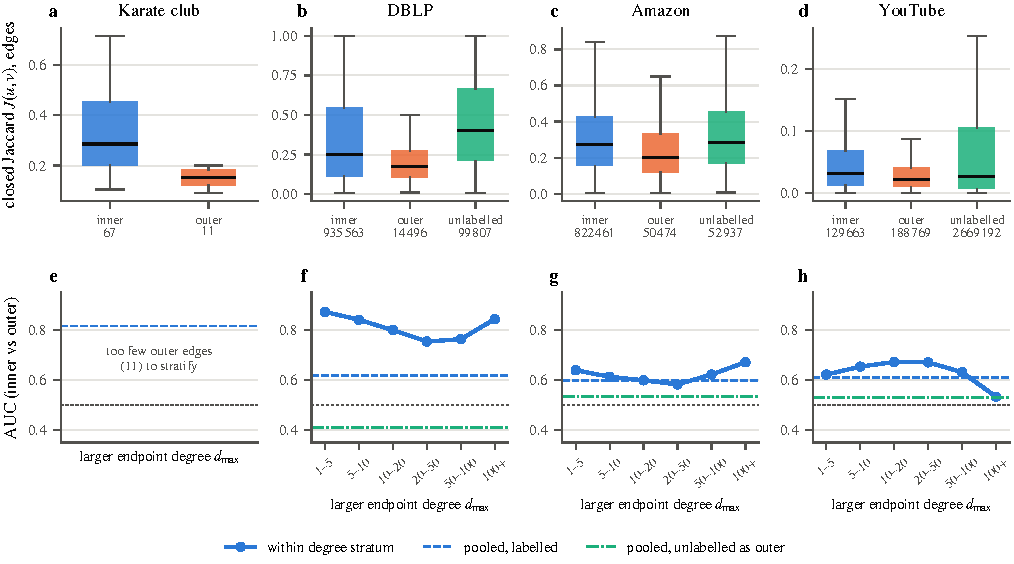
\includegraphics[width=\textwidth]{figures/fig_real_commonality.pdf}
  \caption{Commonality of edges in four networks with recorded memberships.
  (a--d)~Closed-neighbourhood Jaccard of edges whose endpoints share a recorded group
  (inner), are both labelled but share none (outer), or include an unlabelled node;
  boxes span the quartiles, whiskers the 5th--95th percentiles, numbers give edge
  counts. (e--h)~AUC for separating inner from outer edges within strata of the larger
  endpoint degree (points), pooled over all labelled edges (dashed), and with
  unlabelled edges counted as outer (dash-dotted), as in the earlier analysis of
  Ref.~\cite{deinega2023thesis}.}
  \label{fig:S-realcommonality}
\end{figure*}

\begin{figure*}[p]
  \centering
  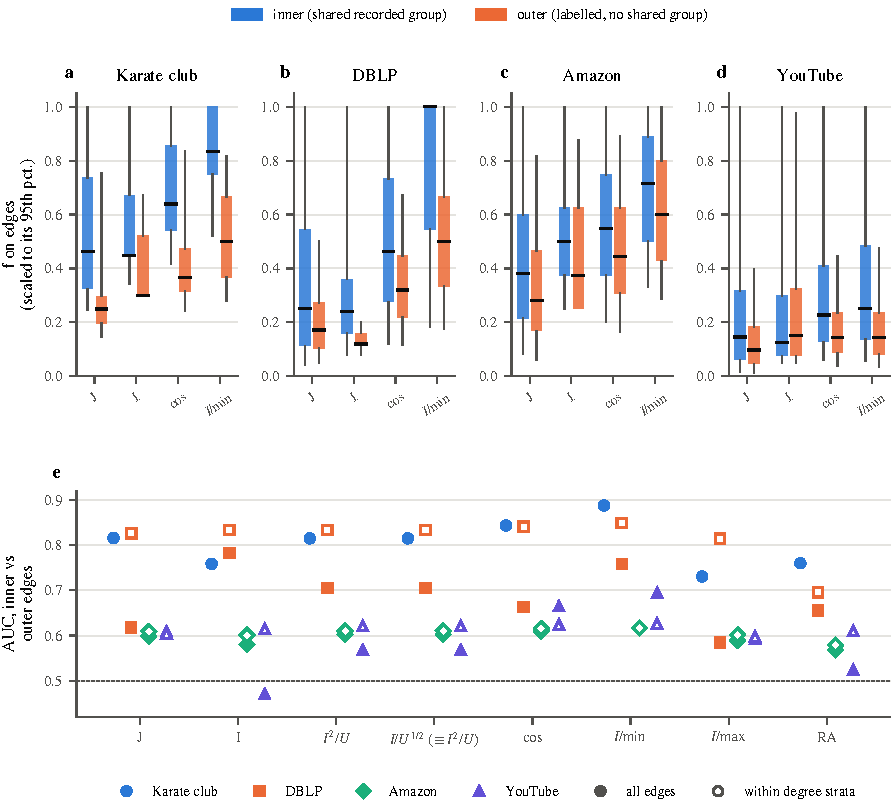
\includegraphics[width=\textwidth]{figures/fig_real_family.pdf}
  \caption{Commonality as a family of functions. (a--d)~Inner (shared recorded group)
  and outer (labelled, no shared group) edges under four functions, each scaled to its
  own 95th percentile. (e)~AUC for separating inner from outer edges with eight scores,
  over all labelled edges (filled) and within strata of both endpoint degrees (open);
  $I/U^{1/2}$ ranks pairs as $I^2/U$ does. The karate club is too small to stratify.}
  \label{fig:realfamily}
\end{figure*}

\begin{figure*}[p]
  \centering
  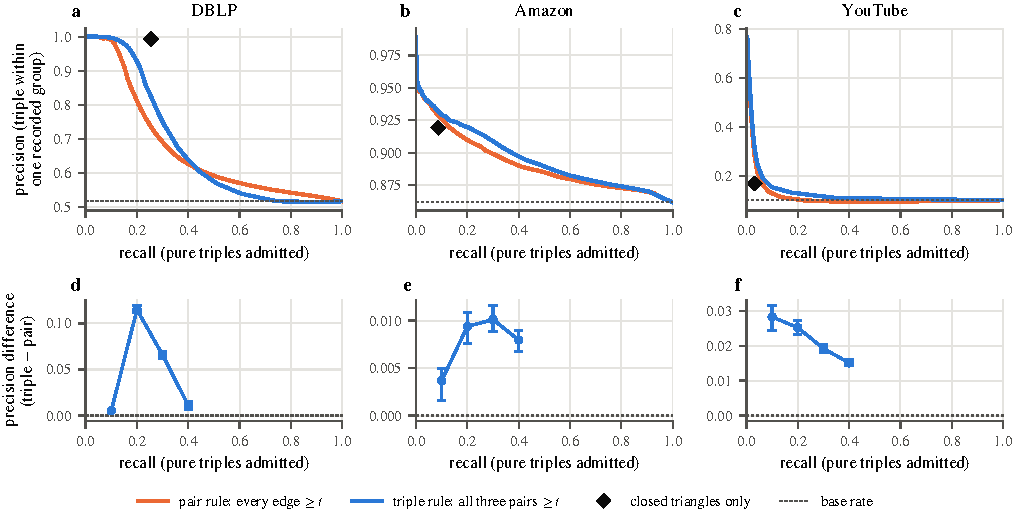
\includegraphics[width=\textwidth]{figures/fig_real_triples.pdf}
  \caption{Pair rule versus triple rule on unique labelled triples (wedges sampled
  uniformly, triangles weighted $1/3$). Precision is the fraction of admitted triples
  contained in one recorded group, recall the fraction of such triples admitted, as
  the threshold varies. Diamond: closed triangles only, without a threshold. Bottom
  row: difference in precision between the triple and the pair rule at equal recall,
  with 95\% intervals from resampling the triples; the y-axes of the top row differ
  between panels.}
  \label{fig:realtriples}
\end{figure*}
